\section{Hipster}%Methodology}
\label{sec: methodology-hipster}


\looseness -1 In this section, we introduce \textbf{Hipster}, a hybrid reinforcement
learning (RL) approach coupled with a feedback controller that dynamically allocates
workloads to heterogeneous cores while selecting optimised DVFS settings.  We propose a
variant, called HipsterIn, that is optimised for latency-critical workloads running solo
in the system, adjusting the system configuration to reduce energy consumption. The
HipsterCo variant, which supports collocation of latency-critical and batch workloads, and
focuses on maximising the throughput of the batch workloads. Both variants of Hipster
always ensure that the QoS requirements are met for the latency-critical workload. 

\subsection{Hipster Reinforcement Learning} \label{subsec:learninng}

The RL problem solved by Hipster is formulated as a Markov Decision Process
(MDP)~\citep{Puterman:1994:MDP:528623}. In an MDP, a decision-making process must learn
the best course of action to maximise its total reward over time.  At each discrete
instant, $n$, the process can observe its current \emph{``state''}, $w_n$, and it must
choose an \emph{``action''} $c_n$ from a finite set of alternatives. Depending on the
chosen action and current state (but nothing else), there is an unknown probability
distribution controlling which state, $w_{n+1}$, it enters next and the reward, $\lambda_n$,
that it receives. The problem is to maximise the total discounted reward, given by
$\sum_{n=0}^{\infty} \gamma^n \lambda_n$, where $\gamma$ is the discounting factor. The
discounting factor $\gamma$ should be positive and (slightly) less than one, in order to
reflect a moderate preference for rewards in the near future. 


\nomenclature[a-wn]{$w_n$}{The current \emph{``state''} in MDP refers to load of the
latency-critical workload measured during time interval $t_{n-1}$ to $t_n$}

\nomenclature[a-cn]{$c_n$}{The action chosen from a finite set of alternatives for the
current state, $w_n$, in time interval $t_{n}$ to $t_{n+1}$} 

\nomenclature[a-wn1]{$w_{n+1}$}{The next \emph{``state''} in MDP based on the current
action, $c_n$} 

\nomenclature[g-tdr]{$\sum_{n=0}^{\infty} \gamma^n \lambda_n$}{The aim of MDP is to maximise
this function, total discounted reward} 


\nomenclature[z-MDP]{MDP}{Markov Decision Process}

\nomenclature[g-lambda]{$\lambda_{n}$}{Positive or negative reward in MDP for the chosen action,
$c_n$ is updated at $t_{n+1}$ }

\nomenclature[g-gamma]{$\gamma$}{Discounting factor in MDP}

\nomenclature[g-xi]{$\xi$}{Learning factor in MDP}

The hybrid task management problem solved by Hipster is translated to an MDP as follows.
The state $w_n$ indicates the current load on the latency-critical workload, measured during the (prior) time interval
$t_{n-1}$ to $t_n$.\footnote{Load is Chapter~\ref{chapter: hipster} (only)
refers to load of the latency-critical workload measured in requests per second, or
queries per second, whereas in Chapter~\ref{chap: REPP} it is referred to as IPS.} Hipster quantises the load into buckets.  Specifically the
latency-critical application provides a measurement of the percentage load during the time
interval, in terms of requests per second, queries per second, or similar. The action,
$c_n$, which is chosen by Hipster depending on the state, determines the configuration to
be used in the (next) time interval, $t_n$ to $t_{n+1}$; that is, the combination of cores
and DVFS settings allocated to the latency-critical application.  These settings are used
for the upcoming interval, at the end of which, at time $t_{n+1}$, the reward $\lambda_n$ is
determined depending on the level of QoS relative to the target, given a metric of
optimisation: either the system power consumption (HipsterIn) or the throughput of the
batch workloads (HipsterCo). A precise definition of the calculation of the reward is
given in Section~\ref{subsec: rewardcalculation}.


RL is a type of unsupervised machine learning with a focus on online
learning~\citep{Mnih2015Human-levelLearning}. It solves an MDP by maintaining a table of
values, $R(w,c)$, indexed on the possible states $w\in W$ and possible actions $c\in C$.
The entry $R(w,c)$ estimates the total discounted reward that will be received, starting
from state $w$, if the decision-making process starts by choosing next action $c$.
Assuming that the \textbf{lookup table}, $R(w,c)$ has close to correct values, then, if
the current state is $w_n$, the best action $c_n$ is the one that gives the largest total
discounted reward; i.e. $c_n = \arg\max_c R(w_n, c)$.  The process chooses this value of
$c_n$, then it updates $R(w_n, c_n)$ using a particular formula based on the old and new
states, $w_n$ and $w_{n+1}$, and the reward $\lambda_n$.\footnote{The update of
$R(w_n,c_n)$ is on line~17 of Algorithm~\ref{pseudo:reward}.} A classic problem in RL is
known as the \textit{exploitation--exploration dilemma}, which captures the need not only
to exploit the best solution identified so far, but also to fully explore alternatives,
which may or may not be better.  

\nomenclature[a-rwc]{$R(w,c)$}{A lookup table of rewards for state $w$ and action $c$}

\nomenclature[a-ba]{$c_n = \arg\max_c R(w_n, c)$}{The action with the highest reward,
$c_n$ among the possible set of actions, $c$, for the current state, $w_n$}


Hipster uses a hybrid RL approach~\citep{TesauroAAllocation}, which combines reinforcement
learning with a heuristic, to be used while the algorithm is still learning the optimal
behaviour. For Hipster, the heuristic improves QoS at the beginning of the execution and
it is also re-used after a change in the characteristics of the problem, e.g.\ the mix of
batch workloads. A hybrid RL~\citep{TesauroAAllocation} has the potential to outperform
pure RL schemes~\citep{2007IBMReports,Tesauro2005OnlineLearning.} that only deal with the
exploitation--exploration dilemma (e.g.\ Q-learning), for several reasons: 

\begin{itemize}

    \looseness -1 \item[{\small \circled{1}}] During the learning phase, online
        unsupervised learning without a heuristic generates random decisions, which would
        produce an unacceptable number of QoS violations.

\looseness -1 \item[{\small \circled{2}}] As the complexity of the problem increases, in
    terms of workloads, number of cores, DVFS settings, and so on, it may take longer to
        learn the table $R$. In contrast, a hybrid RL can find acceptable solutions even
        during the learning phase.

\looseness -1 \item[{\small \circled{3}}] The exploration feature of many RL approaches is
    necessary to capture a global maximum, but it may cause extra QoS violations.  Using a
        heuristic in the learning phase can reduce the need to explore configurations that
        clearly violate QoS.

\end{itemize}


\subsection{Hipster Design}
\label{subsec: design}

\begin{figure}[htbp]
    \centering
    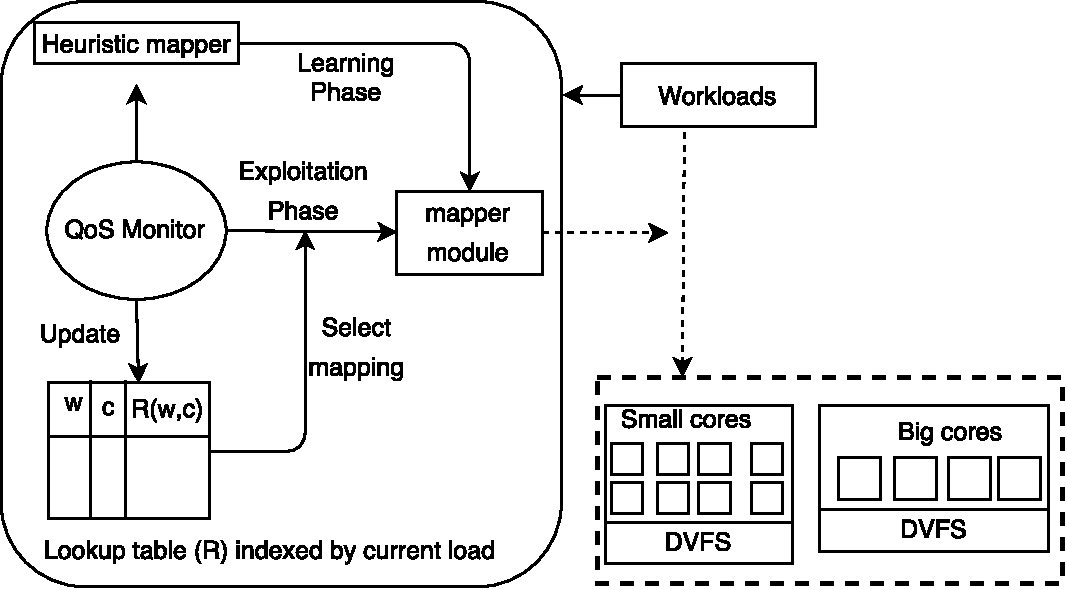
\includegraphics[scale=0.6]{Chapter4/Figs/RIL-Vinson-nocloud-new.pdf}
    \caption{High-level view of Hipster runtime system} 
    \label{fig:hipsteroverview}
\end{figure}

Figure~\ref{fig:hipsteroverview} shows a high-level view of Hipster. Hipster includes a
QoS Monitor, a heuristic mapper (used in the learning phase), an Exploitation Phase, and a
Mapper Module (used in both learning and exploitation phase). Given a QoS target, an
incoming load, and a metric to optimise for, Hipster learns the most adequate core
configuration and DVFS settings by managing a lookup table that is used to map the
workloads to the available hardware resources.

\paragraph*{QoS Monitor.} The QoS Monitor is responsible for periodically collecting the
performance statistics from the latency-critical and batch workloads. For the
latency-critical workload, Hipster gathers the appropriate application-level QoS
metrics such as throughput (RPS or QPS) and latency (query tail latency). It also reads
the current load on the latency-critical workload and quantises this value into discrete
buckets between 0 and $T-1$, for (some) small value $T$. HipsterCo uses a profiling tool
to measure the throughput of the batch workloads, using per core hardware performance
counters, such as CPU utilisation, cache-misses and IPS.

\paragraph*{Learning and exploitation phases.} The data collected by the QoS monitor is used
to make the thread-to-core mapping decisions. In the learning phase, Hipster uses a
feedback control loop based on heuristics to map the latency-critical workload to
resources. Following the intuition from Section~\ref{sec:Motivation}, when load is low,
the mapper executes the latency-critical workload on small cores at lower DVFS states, and
when load is high, it uses a combination of big and small cores at higher DVFS.  Hipster
also begins populating the lookup table so that each entry approximates the corresponding
total discounted reward.  Specifically, Hipster uses the reward mechanism
(Section~\ref{subsec: rewardcalculation}) to prefer core configurations that minimise
system energy consumption or maximise batch workload throughput, while ensuring as well as
possible that at least \SI{95}{\percent} QoS guarantee is achieved~\citep{Horvath2007DynamicControl}.

In the exploitation phase, Hipster uses the lookup table to select the core mapping and
DVFS settings, based on the load. It also continues to update the values in the lookup
table, in order to continue to improve the mapping decisions. At runtime, Hipster
determines when to dynamically switch between the learning and exploitation phases, based
on a prefixed time quantum. At deployment stage, we ensure that the bucket size for each
workload gives at least \SI{95}{\percent} QoS guarantee~\citep{Li2014TalesTail} with minimal energy
consumption.

\subsection{Heuristic Mapper (Learning Phase)}
\label{subsec: hybrid}

The heuristic mapper is a state machine with a feedback control loop. The current state
identifies the core configuration: the DVFS settings and number and type of cores to use
for the latency-critical workload.\footnote{State machines and Markov Decision Processes
use ``state'' with different meanings. In Section~\ref{subsec: hybrid} (only), ``state''
refers to the core configuration, elsewhere it is the load.} The choice of available
states depends on the platform; that is, the total number and types of cores, and the DVFS
settings. There is a predefined ordering of the states, approximately from highest to
lowest power efficiency. This ordering is determined by measuring the power and
performance of each state using a stress microbenchmark consisting of mathematical
operations without memory accesses.

Whenever QoS is close to being violated, the state machine transitions into the
next-higher power state. The QoS is quantified using the currently measured tail latency
at the \ninefive or \ninenine percentile, denoted $QoS$\textsubscript{curr}. The target tail latency
is denoted by $QoS$\textsubscript{target}. The state machine transitions to the
next-higher state whenever the time interval ends in the so-called \emph{danger zone}
defined by:

\begin{equation*}
\label{eq:Death-zone}
QoS_{\mathit{curr}} > QoS_{\mathit{target}} \times QoS_{\mathit{D}}
\end{equation*}


\nomenclature[a-qoscurr]{$QoS_{\mathit{curr}}$}{Currently measured tail latency at the \ninefive or \ninenine percentile for the latency-critical workload}
\nomenclature[a-qostarget]{$QoS_{\mathit{target}}$}{The target tail latency for the latency-critical workload}
\nomenclature[a-qosD]{$QoS_{\mathit{D}}$}{QoS as a factor of a co-efficient between 0 and 1}
\nomenclature[a-qosS]{$QoS_{\mathit{S}}$}{QoS as a factor of a co-efficient between 0 and $QoS_{\mathit{D}}$}

where $QoS_\mathit{D}$ is a parameter between 0 and 1 that defines the size of the danger
zone. Whether such a state transition improves or degrades performance and whether it
actually increases or decreases power depends on the characteristics of the platform and
the particular workloads. The state machine may have to make several consecutive state
transitions until the QoS is met.

In contrast, whenever the QoS is far from being violated, the state machine transitions
into the next-lower power state. This happens whenever the time interval ends in the
so-called \emph{safe zone} defined by:

\begin{equation*}
\label{eq:Safe-zone}
QoS_{\mathit{curr}} < QoS_{\mathit{target}} \times QoS_{\mathit{S}}
\end{equation*}

where $QoS_\mathit{S}$ is a parameter between 0 and $QoS_\mathit{D}$ that defines the size
of the safe zone. The values of $QoS_\mathit{D}$ and $QoS_\mathit{S}$ are determined to
avoid oscillations between adjacent states.  In particular, $QoS_\mathit{D}$ is
empirically computed in the same way as for
Octopus-Man~\citep{Petrucci2015Octopus-Man:Computers,Horvath2007DynamicControl}.

The heuristic proposed by Octopus-Man is attractive because of its simplicity but it can
be sub-optimal (see Section~\ref{sec:Motivation}, Figure~\ref{fig: state-transition})
because there is no common static ordering of configuration states that works for all
workloads. Moreover, in practice, the state machine may respond slowly to rapid changes in
load. Nevertheless, we found that such a state machine heuristic is suitable to accelerate
the learning phase of the RL algorithm by exploring viable core configurations to quickly
populate reasonable values into the lookup table.

%Algorithm 1: Reward mechanism
\begin{algorithm}[t]
  \caption{Reward mechanism}
  \label{pseudo:reward}
  \begin{algorithmic}[1]
    \Statex \Comment{\emph{Determine reward ${\lambda}_n$ based on interval $t_n\dots t_{n+1}$}}
    
    \State Let $QoS\textsubscript{target}$ be the target QoS of the interactive workload.
    \State $QoS\textsubscript{curr}$ = $QoSMonitorLatency$
    \State $Power$ = $QoSMonitorPower$
    \State $QoS\textsubscript{reward}$ = $QoS\textsubscript{curr} / QoS\textsubscript{target} $ 
    \State $Power\textsubscript{reward} = TDP / Power $ \Comment{\emph{TDP (thermal design power)}}
    \If{$QoS\textsubscript{curr} < QoS\textsubscript{target}\times QoS\textsubscript{D}$}
     \State $\lambda_n = QoS\textsubscript{reward} + 1$
    \ElsIf{$QoS\textsubscript{curr} < QoS\textsubscript{target}$}
    \State $\lambda_n = QoS\textsubscript{reward} + 1 - Random(0,1)$ 
    \Else
    \State $\lambda_n = -QoS\textsubscript{reward} - 1$
    \EndIf
    \If{there exist batch jobs}
      \vspace{2mm}
    \State $\lambda_n = \lambda_n + \frac{B\textsubscript{IPS}+S\textsubscript{IPS}}{maxIPS(B) + maxIPS(S)}$
    \Else
	\State $\lambda_n = \lambda_n + Power\textsubscript{reward}$
    \EndIf
    \State \emph{$\mathrm{\mathbf{if}}$ $\nexists$ $R(w_n, c_n)$~$\mathrm{\mathbf{then}}$~$R(w_n, c_n) = 0$}
    \vspace{2mm} 
    \State $R(w_n,c_n) = R(w_n,c_n) + \xi\Big(\lambda_n + \gamma\max_{d\in C}R(w_{n+1},d) - R(w_n,c_n)\Big)$
    
  \end{algorithmic}
\end{algorithm}


\subsection{Reward Calculation}
\label{subsec: rewardcalculation}

During both the learning and exploitation phases, the values in the lookup table are
dependent on the reward, which is calculated as defined in Algorithm~\ref{pseudo:reward}.
This reward calculation is invoked after each monitoring interval, and its definition was
determined empirically (more details in Section~\ref{subsec: respstab}). The reward
$\lambda_n$ has three parts: the QoS Reward, Stochastic Reward, and either the Power
Reward (for HipsterIn) or the Throughput Reward (for HipsterCo):

\paragraph*{QoS Reward.} The ratio of the measured QoS to the QoS target is known as
$QoS_\mathit{reward}$.  If this value is less than one, then the QoS target has been met,
and it quantifies how quick the response was as the \textbf{QoS earliness}. In this case,
line~7 or~9 applies a positive reward that prefers configurations that approach the QoS
target, which acts as a heuristic to reduce energy consumption or improve batch workload
throughput.  If $QoS_\mathit{reward}$ is greater than one, then the QoS target has
\emph{not} been met, and it determines how intense the violation was as the \textbf{QoS
tardiness}. In this case, line~10 applies a negative QoS reward. 

\nomenclature[a-qosr]{$QoS_{\mathit{reward}}$}{The ratio of $QoS_{\mathit{current}}$ to $QoS_{\mathit{target}}$}


\paragraph*{Stochastic Reward.} When the QoS is below the target, as defined in
Section~\ref{subsec: hybrid}, but still over the danger zone, then a stochastic penalty is
applied (line~9 of Algorithm~\ref{pseudo:reward}). The stochastic penalty offers the
possibility to continue to explore the configuration, but with a smaller probability. In
future, other external influences for the latency-critical workload like noise, contention
on shared resources, pending queue lengths, etc., may cause a QoS violation.



\nomenclature[z-tdp]{TDP}{Thermal Design Power}

\nomenclature[a-powerr]{$Power_{\mathit{reward}}$}{The ratio of $TDP$ to $Power$}

\looseness -1  \paragraph*{Throughput Reward (HipsterCo).} Line~13 of
Algorithm~\ref{pseudo:reward} calculates the Throughput Reward, which is approximately
proportional to the total throughput of the batch workloads. Since HipsterCo does not
require modifications to the batch workloads, it is only possible to measure their
throughput in a generic way using performance counters. Specifically, the throughput is
quantified in terms of IPS. The parameters $B\textsubscript{IPS}$ and
$S\textsubscript{IPS}$ measure the total IPS of the big and small clusters running batch
workloads, respectively. The denominator is constant given by the sum of $maxIPS(B)$ and
$maxIPS(S)$, which measure the maximum IPS, at highest DVFS, for the big and small cores
respectively. Platform specific details are given in Chapter~\ref{chap:
infrastructure}.%Section~\ref{subsec: experimental setup}.  

\paragraph*{Power Reward (HipsterIn).} The ratio of the thermal design power (TDP) to the
measured system power consumption is known as $Power_{\mathit{reward}}$ as shown in
line~15. A smaller value of this term means that the system power consumption was lower,
and it increases the reward. 

\vspace{1.5mm}

Once the reward $\lambda_n$ has been calculated, line~17 updates the value of $R(w_n,
c_n)$ in the lookup table, and this is done in the same way during both the learning and
exploitation phases. This update is controlled using two scalar parameters, both between
zero and one: the learning rate, $\xi$, and, the discounting factor, $\gamma$.

\looseness -1 \paragraph*{Learning Factor, $\xi$.} The $\xi$ coefficient in line~17 of
Algorithm~\ref{pseudo:reward} is the learning factor, which controls the rate at which the
values in the lookup table $R(w,c)$ are updated. A large value of $\xi$ close to one means
that the algorithm learns quickly, favouring recent experience, but increasing
susceptibility to noise. In contrast, a small value of $\xi$ means that the algorithm
learns slowly. In our experiments we used $\xi=0.6$. 

\paragraph*{Discounting Factor, $\gamma$.} The $\gamma$ coefficient in line~17 of
Algorithm~\ref{pseudo:reward} is the discounting factor, which quantifies the preference
for short-term rewards~\citep{Suton.R.S1998ReinforcementIntroduction}. Setting $\gamma=0$
means that the algorithm only relies on immediate short-term rewards. To allow a
balance between short-term and future rewards, we set $\gamma=0.9$ (empirically
determined). In other words, this methodology allows the optimization problem to also
take into account future rewards.



% Algorithm 2: Exploitation phase
\begin{algorithm}[tb]
  \caption{Exploitation Phase}
  \label{pseudo:callreward}
  \begin{algorithmic}[1]
    \State Let $X$ be threshold on QoS guarantee to re-enter learning phase
    \State Let $w_n$ be observed load for interval $t_{n-1}\dots t_n$
    \State Let $c_n$ be configuration for interval $t_n \dots t_{n+1}$
    %\State Let $R(w,c) = 0$ for all $w$, $c$
    \State Let $n = 0$
    \Repeat 

    \Statex \Comment{\emph{At time $t_n$, choose configuration for $t_n$ to $t_{n+1}$}}
    \State Let $c_n = max_{d\in C}R(w_n,d)$	

    \If{there exist batch jobs}
		\State Allocate remaining cores to batch jobs
    	\If{latency-critical jobs on a single core type}
        \State Set highest DVFS for other core type
        \EndIf
     \Else
     	\State Set lowest DVFS for remaining cores     
     \EndIf

     	\State Sleep until $t_{n+1}$  \Comment{\emph{Run for interval $t_n$ to $t_{n+1}$}}
        \State Let $w_{n+1}$ be the quantised load from the latency-critical workload
        \State Call Algorithm~\ref{pseudo:reward} \Comment{\emph{Algorithm~\ref{pseudo:reward} updates $R(w_n,c_n)$}}
    \State $n = n+1$
    
    \State {\textbf{if} $QoS Guarantee \leq X$ \textbf{then} Learning phase}
    \Until{Terminated}
  \end{algorithmic}
\end{algorithm}


\subsection{Exploitation Phase}
\label{subsec: exploitation}

The exploitation phase of Hipster is defined by Algorithm~\ref{pseudo:callreward}. Line~6
determines the configuration, $c_n$, with the highest estimated total discounted reward.
Lines~7 to~12 apply the configuration by mapping the workloads to the resources, as
described below, depending on the specific variant of Hipster (HipsterIn or HipsterCo).
Line~13 runs the workload for the next time interval, and line~15 calls
Algorithm~\ref{pseudo:reward} to update the lookup table, based on the metrics obtained by
the QoS Monitor during the time interval. Line~17 re-enters the learning phase when
necessary.  The mapping of workloads to resources is as follows:

%Need to describe Line~7

\paragraph*{Reward Mechanism for HipsterIn.} To minimise power consumption while meeting
the QoS target for latency-critical workloads, the configuration with the highest reward
is selected and then DVFS setting for the remaining cores is set to the lowest value
(Lines~11 to~12 of Algorithm~\ref{pseudo:callreward}).

\paragraph*{Reward Mechanism for HipsterCo.} Corroborating the findings of prior
work~\citep{Lo2015Heracles}, we observed that collocating both latency-critical and batch
workloads degrades QoS at higher loads due to shared resource contention. If the reward
mechanism were not aware of such collocations, it may make decisions that violate QoS for
the latency-critical workload and/or reduce the throughput of the batch workloads.  As a
precursor to this condition, we introduce the following mechanisms. First, to maximise the
throughput of the throughput-oriented workloads while meeting QoS targets, all of the
unused cores are allocated to the batch workloads (lines~7 to~8 in
Algorithm~\ref{pseudo:callreward}). Second, in case the latency-critical job is allocated
exclusively to a given core type, the other core type is set to the highest DVFS to
accelerate the batch workloads (lines~9 to~12 in Algorithm~\ref{pseudo:callreward}). For
instance, on a two-socket/cluster system with two cores per socket/cluster, if the
latency-critical workload is running on two small cores, the big cores are allocated to
the batch workloads at the highest DVFS. 

\subsection{Responsiveness and Stability}
\label{subsec: respstab}

\looseness -1 To ensure that QoS is met for latency-critical workloads, the scheduling policy must
quickly respond to fluctuations in load and latency, either due to changes in core
mapping, DVFS or any external influence. Therefore, the responsiveness and stability of
Hipster is determined by {\small {\circled{1}}} the computation latency in migrating cores and setting DVFS.
{\small {\circled{2}}} the reaction time of QoS between migrating an application from current mapping to
future mapping, and {\small {\circled{3}}} the granularity of monitoring for the latency-critical workload's
QoS. 

The computational latency for changes in core mapping and DVFS are
negligible~\citep{Cong2012Energy-efficientArchitectures, Leverich2009PowerGating, Madan2011AProcessorsb}.
The default monitoring interval for Memcached and Web-Search is one second. Based on the
aforementioned overheads, we determine the  sampling interval as a sum of the monitoring
interval for the latency-critical application, and the overhead to switch the core mapping
and DVFS.


\subsection{Hipster Implementation}
\label{subsec: implementation}

Hipster is implemented in user space, and it uses minimal hardware support exposed by
Linux. It consists of the QoS Monitor and Mapper Module, together with a lookup table, as
shown in Figure~\ref{fig:hipsteroverview}. 

\looseness -1 \paragraph{QoS Monitor.} Hipster uses a separate process to read the power measurements
using native energy meters, at the sampling interval of the application. In addition to
measuring energy, the QoS Monitor also gathers runtime statistics for the query/request
latency of the latency-critical workload, using a logfile interface. In the case of
HipsterCo, the  batch workload aggregate IPS per core are measured using the performance
monitoring tool, \textsf{perf}~\citep{2016Perf:Counters}, specifically using the
\textit{perf\_event}
\textsf{instructions}~\citep{ARMLimitedARMManual,ARMLimitedARMManualb}. Alternatives to
\textsf{perf} include the profiling tools~\citep{Ren2010Google-WideCenters,
Kanev:2015:PWC:2749469.2750392} supported by Docker, Kubernetes and
LXC~\citep{Bernstein2014ContainersKubernetes}.  

As discussed in Section~\ref{sec: perfmon thesis}, the \textsf{perf} bug on ARM processors
generates garbage values for all cores whenever any core enters an idle state.  Since
performance statistics are required only necessary for the HipsterCo variant (where batch
workloads are collocated with latency-critical workloads), we overcome this by disabling
the CPUidle. 

\vspace{-2mm}

\looseness -1 \paragraph{Mapper Module.} The workloads are mapped to cores using the Linux
\textsf{sched\_setaffinity} call and DVFS is controlled using \textsf{acpi-cpufreq}. In
addition, Hipster suspends and resumes the batch workloads using the relevant OS signals
({\small \textsf{SIGSTOP}} and {\small \textsf{SIGCONT}} in Linux).

\vspace{-1mm}

\looseness -1 \paragraph{Runtime overhead.} Hipster has a simple algorithm, requiring few control flow
statements and main memory accesses, so its runtime overhead is negligible.  We measured
the execution time overhead (implemented in Python and including I/O) to be $<$ \enspace
\SI{2}{\milli\second}, so triggering Hipster every second, as in our experiments, incurs
an overhead $<$ \enspace \SI{0.2}{\percent}.

\begin{wrapfigure}{r}{0.45\textwidth}
%    \centering
    \vspace{-17mm}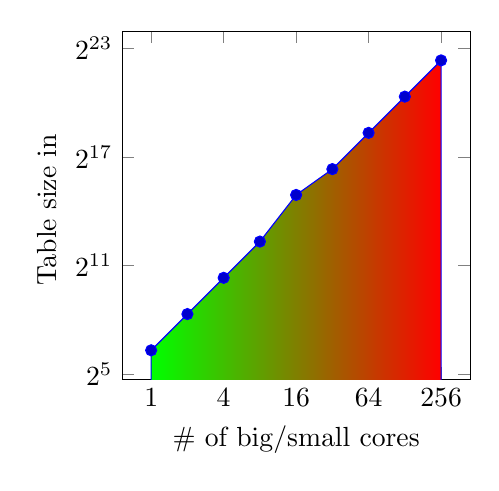
\begin{tikzpicture}
    \begin{axis}[
            xlabel= {\# of big/small cores},
            ylabel= {Table size in $\SI{}{\kilo\byte}$},
            ymode=log,
            log basis y={2},
            enlarge x limits=0.1,
            legend style={
                    at={(0.5,-0.15)},               
                    anchor=north,legend columns=-1
            },
            width=6cm,
            height=6cm,
            point meta={x},
            symbolic x coords={1, 2, 4, 8, 16, 32, 64, 128, 256},
    ]
    \addplot+  [left color=green, right color=red] coordinates {
        (1, 80) (2, 320) (4, 1280) (8, 5120) (16, 30480) (32, 81920) (64, 327680) (128, 1310720) (256, 5242880) } \closedcycle;
    \end{axis}
    \end{tikzpicture}
    \vspace{0mm}
    \caption[Lookup table size in \SI{}{\kilo\byte}]{Lookup table size (log scale) with same number of small and big cores, using 10 different DVFS settings, and bucket size of 100.}
    \vspace{-3mm}
    %\vp{X axis should change "\# of big cores" to "\# of big/small cores"}
    \label{fig:size}
\end{wrapfigure}

\looseness -1 \paragraph{Lookup table.} Each iteration of the RL algorithm accesses and modifies several
entries in the lookup table. To ensure that these operations take negligible time, the
computational complexity to access the table should be at most a few instructions.
Therefore, in the prototype implementation of Hipster, the lookup table was implemented
using a Python dictionary, which uses open addressing to resolve hash collisions, thereby
having a computational complexity of $\mathcal{O}(1)$ irrespective of the
operation~\citep{PattisComplexityHttps://www.ics.uci.edu/pattis/ICS-33/lectures/complexitypython.txt}.

\looseness -1 We observe that the lookup table size can grow quickly (see Figure~\ref{fig:size}) with
the number of big/small cores, DVFS settings, and the number of load buckets. Let us say
there are $B$ big cores and $S$ small cores available, and $B_{f}$ and $S_{f}$ available
DVFS settings for big and small cores, respectively, then the total number of actions in
the table would be $C$($B$+$B_{f}$, $B_{f}$) $\times$ $C$($S$+$S_{f}$, $S_{f}$), where
$C$(x, y) refers to the number of different ways to choose actions ($y$) for out of $x$
distinct elements. This grows in the order of $\mathcal{O}(B^{B_{f}} \times S^{S_{f}})$.



\looseness -1 Figure~\ref{fig:size} shows the unoptimised (or na\"{\i}ve) lookup table size in
\SI{}{\kilo\byte} when the number of big cores is equal to number of small cores ($B$ =
$S$) with 10 DVFS states for big and small cores ($B_{f}$ = $S_{f}$ = 10) with 100 load
buckets ($w$). For instance, 64 cores of each type leads to 40,960,000 combinations (in
contrast to 56 configurations on ARM Juno), which gives a table size of approximately
$\SI{327}{\mega\byte}$ for a whole node.  

To reduce the size of the lookup table in Hipster, we store the configuration and reward
only for the configurations which have been explored so far. The lookup table is still
implemented using a Python dictionary as the complexity is $\mathcal{O}(1)$ irrespective
of the operation. Furthermore, in the exploitation phase, we ensure that each load bucket
($w$) contains \emph{only} the top $K$ (in our case, $K=5$) configurations with highest
discounted maximum rewards. 

